\section{Timeline}

The following section describes the project development, progress and decision as we did through the time the the project was developed. After series of informal talk the project officially started in December 2011 and was submitted in September 2012.

\subsection{Initial project meetings and early implementation decisions}

The regular project meeting where we discussed mostly the organizational aspects and the top-level design of the application started in December 2011. We easily agreed that we were aiming to create an application quite similar to the Google Documents. We have decided very early to use the multi tier architecture consisting of

\begin{itemize}
\item core translation memory,
\item user space,
\item graphical user interface,
\end{itemize}

which became very soon separate Maven modules (as soon started using Maven for building the project). Despite we added further modules later, we consistently kept the initial project splitting into \emph{Core}, \emph{User Space} and \emph{GUI}. At the beginning we also assigned team members to the different part of project which remained surprisingly stable as well. 

Before receiving the data from OpenSubtitles.org we were thinking about the source of data to fill the translation memory for the first time. There were several options -- either using the subtitle part of the Czech-English parallel corpus CzEng developed at ÚFAL, using sentences from a general purpose parallel corpus or getting the data from a subtitle server.

From the very beginning we intended base the project on Java. Mainly because there exist quite a lot of web technologies based on Java and everybody of us were at least a little bit familiar with it. We also decided to combine the code in Java and Scala programming languages and Apache Maven as a build manager. At that time there was only one team member who knew the Scala language. Despite we repetitively expressed believes that everybody of would learn it, at the end there was one another person familiar with the Scala language which appeared to be a bottleneck of work on the translation memory core.

Much complicated was to agree on the technology of the client. There were many different opinions from writing the client in {\it PHP} with {\it Nette Framework} which some of us know quite well, using the {\it JSP} to have all the code consistently in Java or even quite extreme idea to make the whole application as {\it Java Applet} (this idea had appeared because of the intention to integrate the video player in the application and at that time we didn't of any other option of doing it except making a Java applet for it). Finally we decided to use {\it Google Web Toolkit} which nobody of us had had any prior knowledge before, but it promised making the communication between server and client very easy. Similarly to the Scala language we ended up with just two people able to work effectively with the Google Web Toolkit. Fortunately, it did not became a bottleneck of the development process. 

After overcoming the problems connected with learning a new technology we became quite satisfied with the decisions because the usage of Google Web Toolkit and other modules, as well as the possibility to combine all parts of the project with Apache Maven were helpful despite making the project run in Maven was very painful for us and we spent unnecessarily a lot of time by solving this issues.
	
The decision to use both Java and Scala appeared to be a bring quite a lot of complications. On the one hand, Scala allowed to write concise and efficient code, on the other hand most project members were not able to learn Scala sufficiently and hence used only Java. Although the interoperability between Scala and Java works well in most cases because both are based on the JVM, some problems remain. One of the problems of interoperability was, for example, that the implementation of the data type \emph{List} that was created in Scala was not compatible with Google Web Toolkit, which expected a standard Java \emph{List} implementation.

\subsection{Early development process}

Luckily for us we received very soon a database from the {\it opensubtitles.org} containing all the Czech and English subtitle file that were at the server at that time. Soon after that we started an alignment algorithm to retrieve the parallel data from the subtitle files (the process is described in section~\ref{sec:aligning_subtitles}) and enable us to start experiments that helped us to decide which database system could be used.

Choosing appropriate database system was also intensively discussed issue. The database underlying the Translation Memory plays a crucial role for the whole system performance. Also using built-in features could save us a lot of additional work.  We evaluated different DBMS and decided to use Postgres (see section~\ref{sec:dbms} for details). Not having any experience with the object-relation mapping libraries in Java we started to us {\it Hibernate} based on the Internet forums and advice of our colleagues.

Originally, all the algorithms precessing the data we retrieved were implemented in Perl the and the code importing the data were in the \emph{Core} module implemented in Scala. Later, to be the code more consistent, we decided to move the data preparation and data import to a separate \emph{dataimport} module and re-implement the Perl scripts in Scala.

\begin{figure}[h]
\begin{center}
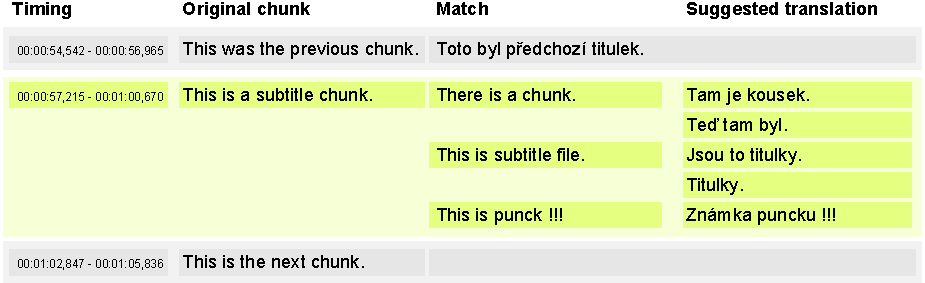
\includegraphics{./figures/original_strucutre.pdf}
\end{center}

\caption{Scheme of the originally intended structure of work with the translation memory. It reflects the original User Space structure and also schematically the original client design.}\label{fig:original_scheme}

\end{figure}

We started to solve very soon the video playback in the browser which we expected to be a really challenging issue. ... we thought about flash, creating application wrapper where an web would be included ...

We very soon had toy implementations of:

- a player using VLC plugin, to be incorporated into the web app

- a player as a desktop java app, showing the web app in a frame

We decided for the web app only version, with no desktop variant, because, observing the development trends, it seems to us that the present and future of applications is in web applications. The benefits are e.g. that the learning curve is typically better for a web application, where the user is already familiar with most of the controls and work patterns, installation is not required so anyone can start using the application immediately, it is easy to use OpenID registration... Disadvantages: cross browser support, limited power, larger bandwith consumption. GWT added advanatage: the bandwith consumption is closer to that of a standalone desktop app, because the application itself is stored in one Javascript file, which is downloaded at the beginning (similar to installing a desktop application), and the rest of the client-server interaction is done through RPCs (basically the same way as it would be done in a desktop application).

\subsection{Introducing the shared classes}

After having implemented very basic version of both three parts of the project we decided it was time to start to solve the interoperability of individual parts in order run a first snapshot of the application. This was happening approximately in March 2012.

At this stage we found out that we are not fully taking advantage of using the Java technologies for all parts of project and decided to totally redesign the User Space and Client parts.

Originally we wanted to keep the traditional translation memory structure where each sentence can have several matches and these matches can have several translations in the memory as is depicted in the figure \ref{fig:original_scheme}. Anyway, this scheme did not reflect much the way we worked with the data in the that time -- suitable matches were provided from the table of translation pairs based on indexes built over the table. Moreover, the were very few matches having more different translations in the data and the design of the GUI of the application was a little bit confusing because it used to place the text of matches to prominent place despite the user is not as concerned about the matches as he is about the actual translation suggestions. This lead to a scheme which is depicted in figure \ref{fig:new_scheme}.

\begin{figure}
\begin{center}
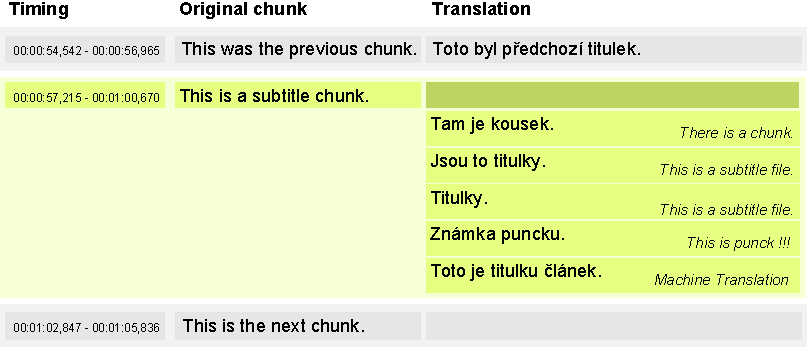
\includegraphics{./figures/current_strucutre.pdf}
\end{center}
\caption{Current scheme of the work with translation memory.}\label{fig:new_scheme}
\end{figure}

We agreed on the shared classes that all parts of the project should use.  We more or less adopted the design of the class from the core and started to use in the whole project. This step required to re-implement the classes from Scala to Java and to drop a lot of code that was already done in the User Space and the client. The design of the classes was almost the same as is described in \ref{sec:shared_structure}.

We started the work on the project with new design soon, anyway it started the period of the biggest struggle with technologies. It took almost two months to have a first running version of the application.

The very first version of the application was a page where it was possible to upload a subtitle file do the translation without any possibility load an already saved subtitle document or download a result of the translation. without any sessions, user, it was just a page, where you edit the subtitles. At that time we used machine translation from the MyMemory service which is in fact Google Translate, anyway there is a limited acces per IP address, so it became obvious the we would have to change the source of machine translation. We used API of IMDB.com, to receive information about movies but the movie meta data was not used in the evaluation the matches at that time.

From the later view it appeared to be an important decision to agree on the shared classes which made the cooperation between the modules easier and less verbose. 

\subsection{???}

Sessions, logging, troubles with OpenID, trying JOpenID, openid4java 

Use our own Moses trained on the subtitle data we have from opensubtitles

\subsubsection{OpenID}

TODO -- Jindra?

we use this and this library because...

we support Google, Yahoo and Seznam because...

we do not support generic openid because the lib does not support this

\subsubsection{Chunk Splitting}

TODO

ideas:

keep as it is, i.e. one timing = one chunk ... too long, too arbitrary

split into sentences, joining already split sentences together ... very hard (probably impossible) to do reliably, would miss the advantage of subtitle files for alignment

now: keep already existing splits, split on dialogue boundaries, slit on sentence boundaries (+ clean away irrelevant characters)

... easy enough to do reliably (SOME NUMBER of errors)

... arbitrary but not so much as the first solution

... length is reasonable

Important: to do the splitting in the same way when creating the database and when processing the user subtitles.
Therefore: a shared Parser class which is compiled both into java bytecode and used in impoting, and into Javascript and used in GUI

\subsubsection{Chunk Time Format}

TODO

we used strings

then we needed to parse these for player and for editing the timing

decided to use the SRT format only (99\% of subtitles we have and easier to use)

a class (SrtTime) that represents the time as a set of integers, providing constructors, getters and setters for all formats we need -- one string, a set of strings, a set of integers, one integer (the time in miliseconds), + compareTo, + subtract

\subsubsection{Chunk Annotations}

TODO

named entities = first reason for annotations

chunk splitting by dashes denoting individual dialogue speekers: dashes need to be removed for translation suggestions generating because they are irrelevat but need be kept for correct rendering of text -> annotations extended to contain dialogue dashes

need to identify the newlines (irrelevant for translation suggestions but necessary to render the subtitles properly) -> annotations extended for newlines

subtitle formatting for bold, italic, underline etc. Original idea: extended the annotations again (easy to do). Then: too much trouble, expecially for GUI. Decision: just strip off these, do not support that. Reasoning: used very little, no formal specification so has various formats, often the players do not support the formatting properly so we want to discourage the users from using the formatting

chunk now has a set of methods to get and set the chunk and annotations correctly, using the notion of FORMS. The forms used are:

database form: the text as stored in the subtitle file, only cleaned -- formatting stripped off (bold, italic etc.), non-printable characters turned into spaces, multiple spaces replaced by one space only... The newlines are stored as PIPE characters.

surface form + annotations: the surface form is the text to be used to generate the translation suggestions, without dashes and with newline turned into spaces

GUI form: HTML form to be displayed in GUI, i.e. newlines turned into BR tags

text form: to be used in textarea -- with dashes, newlines as BACKSHLASH N characters

\subsubsection{Logging}

In US: easy, we use (whatever we use)


In GUI: tricky -- we do not have any "console" so we cannot simply write logs to "standard output"
(actually we have a console, but only in dev mode)

preliminary solutions: "debug prints" ensured by alerts, changing the page title, changing the page statusbar -- not usable in larger scale

development solution: a debug window at the bottom of the page, and a (in the end) static method Gui.log(String) that prints the log messages into that window
... proved to be very useful, with a large enough amount of logging we were often able to locate the bugs from the contents of this window

also added an exception catcher which gets the stacktrace from the exception, then extended to handle umbrella exceptions as well (= multiple exceptions in one)

great: GWT provides stacktraces with filenames and line numbers from the source java code
downpoint: not very reliable but usually useful

great: GWT provides a possibility to catch all exceptions -- using GWT.setUncaughtExceptionHandler() -- it has no real "main" so one cannot just put that into a try-catch block

issue with debug window: cannot appear in final application :-) but still there might be errors;
also it is at the user side, but we need the logs at the server side;
ultimate solution: "remote logging", i.e. important messages are sent to the server through an RPC, where they are both included into the server log and saved into DB for possible future use (together with user id)
The minimal level of a meesage to be sent to the server can be set (debug, info, warn, error)

\subsubsection{Implementing the RPCs}

From the start it was obvious to us that we want to use a well-estabilished method to implement the Remode Procedure Calls. Our first idea was to directly send and receive JSON messages because they have a format of a Javascript object, so we thought that this would be easy and efficient to implement in GWT (it is possible to read the object from string into memore simply using Javascript eval() function). However, there are three facts that we later found out that made us change our decision. The first one is that, although it is possible to directly use eval() function to convert the JSON message into the in-memory object representation, this practice is not recommended for security reasons (any Javascript code can be injected and it would be directly executed with no constraints). Therefore, the recommended practice is to use a JSON parser, which validates the JSON object before calling eval(). A related issue is that although GWT sometimes does use JSON internally, it does not provide a JSON parser to be used by the programmer, so one has to use an additional library. And finally, we found out that GWT already implements a mechanism to send RPCs (in which, as a matter of fact, the messages are actually serialized to JSON).

The type of an RPC parameter or return value can be any GWT-compilable type. Because this type must be known both to the server and to the client, we use only primitive types and shared classes SEE XXX. Each class sendable through GWT RPC mechanism must implement the GWT IsSerializable interface (which is only a marker, i.e. it does not have any abstract methods) and a parameter-less constructor; this also holds for the checked exceptions, which are technically only a special type of a return value.

Because of Javascript and browser limitations, the RPC mechanism of GWT only allows asynchronous calls from client to server. This suited our needs often, but we had to go around these limits in some situations. Quite often we need the RPC to be synchronous and blocking, e.g. in logging in or changing user settings. In such situations, the page or dialog is "deactivated" on invoking the RPC (all active components are disabled -- e.g. the textboxes are read-only, the buttons do not respond to clicks), a reference to the page or dialog is passed to the class invoking the RPC, and when the RPC returns, the page or dialog is "reactivated", either with a success message or an error message, depending on the result of the RPC.

In one case, we would need an opposite direction RPC, i.e. the server to invoke the RPC on the client. This is when authenticating the user through OpenID, where we have to perform the authentiation in a new window -- the new window then receives the result of the authentication, but it cannot be easily passed directly into the opener window. Here we decided to use active polling -- the opener window regularly invokes the GetSessionID RPC, which returns null if the authentication process has not yet finished, this being a signal for the GUI to continue polling.

Most of the RPCs contain the SessionID as one of their parameters to authenticate the user. All of such RPCs can thus throw an InvalidSessionIdException, to which the default GUI action is to show the Login Dialog to the user.

\subsubsection{Failed RPC Requests Handling}

Originally, all the RPC requests followed the barebone AsyncCallback interface, where the request is sent to the server, and onSuccess() or onFailure() method of the callback are called once it returns, depending on the result. The default implementation of onFailure() was to display the error message to the user, the idea behind being that it is eiher a mistake of the user that he should be informed about, or a mistake of the server which he should be informed about as well. This was sufficient for most of the cases; however, it became clear to us that time to time, the requests fail for various reasons beyond our reach (usually temporary network problems), where the default behavior of simply informing the user (and usually throwing away the data he generated for the request) is often not welcome.

We decided that our general error handling strategy should be to try to solve all problems without user interaction, and to inform the user only about user-generated errors (such as incorrect SRT file format or session timeout) or critical errors (such as permanent loss of connection to server).

The first thing was to turn the calls from methods into objects, so that they store their parameters and can be called again on failure. We also created a generic superclass for them, Callable, filled with necessary boilerplate code and methods performing the default actions, to be overridden if necessary. If the request fails for any reason, it is retried by default; four attempts are made for each request, always retrying after a short time interval. We identified the response that we usually get in case of network problems (which could be temporary or permanent), in such case the request is always resent three times. Otherwise, resending the request is the default behavior which the subclasses override in cases where it is obvious that resending will not help (e.g. incorrect e-mail address format or an already existing username on registration). We also added a timeout for each request after which the request is regarded as lost and is retried.

The subclass can always intervene by overriding several methods, such as onSuccessAfterLog, onEachReturn, onFailureAfterLog, onProbablyOffline etc. This way, the behavior needed can be always achieved, but the default implementation is often sufficient, so the subclasses often override only one or two methods, keeping their code as simple as possible. The superclass also provides logging for all the requests, based on the classname and the parameters of the subclass.
(E.g. when deleting a document, a failure with an InvalidDocumentIdException, meaning that the document does not exist, is an error, but there is no need to inform the user because the result is the same as if the RPC succeeded: the document does not exist now.)

\subsubsection{Sending Translation Results}

At first, the translation suggestions from the Translation Memory were requested and sent for each chunk individually. This had the theoretical advantage that the user received each of the translation suggestins as soon as possible. However, we found the overhead of the RPC calls to be unreasonable. Not only was the overall time necessary to load all the suggestions too long, but also a typical browser was unable to handle such a large number of requests and usually froze for long periods of time, often unfreezing only after all of the suggestions arrived.

A simple solution seemed to be sending all of the chunks for translation in one request. However, such a request can take several minutes to complete, and we still wanted to keep the nice property of the application showing the suggestions as soon as possible at least for the first lines -- so that the user can start the translation immediately. Thus, we decided to send the request in batches, starting with a small size of the batch for the beginning of the file and gradually increasing the batch size.

The first way to do that was an exponential increase, where each batch contains twice as many chunks as the previous one, starting with a batch of size one. This proved to solve the aforementioned problem of browser freezing; however, another problem arose. As the batch sizes grew larger and larger, the later requests often took several tens of seconds or even minutes to complete. Meanwhile, the user would often navigate away from the Translation Workspace, rendering the translation suggestions, including the currently being processed ones, obsolete. This was of course detected in GUI and the suggestions were thrown away on arrival, but still it meant that the server was working in vain for some time, possibly resulting in an unnecessarily slower responsiveness to other users (and even to the very same user as well).

We introduced two further solutions. The first and simple one was limiting the size of the batch to 64 chunks (which typically only take about ??? seconds to process), so that the amount of useless work could not grow too large. The second one, which took us some time to think up and implement, was to stop the translation suggestions from being generated on the server, by issuing a StopTranslationResults request. (This breaks the typical model of procesing the queries, where once a query is sent, its processing is not influenced by queries that arrive later.)

The two major issues with the StopTranslationResults request were:

- to interrupt the suggestions generating which is already in process (which is done in parallel for the chunks in the batch, making this even harder).

- to identify what to stop and what to let continue.

The first idea was to mark the whole document as closed, and to check this when generating the suggestions. However, this would cause problems if the same document was immediately reopened by the user, and even larger problems if the user already had the document opened twice -- this can easily happen by mistake, the logical reaction of the user is then to close one of the Translation Workspaces, and then he would stop receiving suggestions even in the other opened Workspace. Thus, we then decided to create an identifier for each Translation Workspace instance and to bind the StopTranslationResults request to this identifier. However, we soon found out that this would require a lot of overhead only to handle this probably not very common situation, so we dropped that idea as well.

Finally, we decided for a compromise solution between those two. The StopTranslationResults request is now bound to individual chunks, which now have an added boolean field isActive. This field is set to true when the GetTranslationResults request arrives to the server, for each of the chunks on the request. The StopTranslationResults request contains a list of the chunks which translations should be stopped. On arrival of that request, Userspace simply sets the isActive field to false -- because Userspace and Core share the same memory and because only references to the chunks are passed around, this change is visible in core even though the chunks have already been sent for translation. The necessary overhead is minimal, and there is no "false alarm" in the typical case. The only unsolved case is the situation where the same batch of chunks are sent for translation at the same time from two different instances of Trabslation Workspace with the same document opened, and then one of these Workspaces is closed, causing the suggestions generation to stop even for the batch from the other Workspace. Although this situation is unlikely and non-critical (the suggestions would be missing only for this one batch, the later batches would be translated correctly), we still offer a general solution by repeating all request on failure (unless it is obvious that the failure will reoccur).

\subsubsection{User Management}

deciding between "simple" login and OpenID ... decided to use both

TODO some notes on OpenID (probably a separate subsetion)

decisions:

no constraints on username (except for non-emptiness)

little constraints on password (only must be >= 3 characters). Resoning:

- we think the most important feature of a password is for the user to remember it, we leave the assessment of the strenght to the user.
often the password strenght constraints are rather arbitrary and many classes of strong passwords do not pass them, it is hard to develop a reasonable strength measure. E.g. a whole sentence, a "passphrase", is a very strong password; however, it usually does not pass measures requiring use of specific classes of characters. And vice versa, a password using very unusual characters (e.g. Czech letters with diacritic signs) can be impossible to break even if it is quite short, because the attacker simply does not try out such characters that are uncommon in passwords; still it often does not pass typical minimum password length constraints.

- the app does not contain any sensitive data whose compromising would pose a threat to the users of the app

- the benefit to the attacker succesfully breaking into a user account is close to none


We allow the user to work in multiple browser tabs or windows, provided it is the same session (i.e. has the same SessionID), because we believe it is natural to work on multiple translations at once, to have the Document List opened to see the translation progres, etc. The user himself is responsible for having the same document opened multiple times, which is not expected behavior and so changes to the document in one Translation Workspace are not projected into the other Workspace until reload.

However, we decided to disallow one user having multiple sessions at one time, as we believe that this is neither expected nor required behavior, and could potentially confuse the user. We believe that such a state is usually caused by a mistake, e.g. user A forgetting to log out on PC 1, then moving to PC 2, and at the same time user B using the application on PC 1 under user A's account by mistake.
We do not support multiple users collaborating on one subtitle file.

If user registers through OpenID, we have to assign a username to him (the unique OpenID identifier we get is typically a long hash, which does not look like a nice username). SEE XXX

Because the username is at least partly generated, the user might not like it. Therefore, we offer each user the possibility to change the username (provided that the one he chooses is free). The username is only used to authenticate the user (if not using OpenID login) and is displayed in the top right corner in the application; the internal unique identifier of a user is his user id, an integer assigned to each user on registration that never changes.

\subsubsection{E-mail Address Validation}

TODO: write it here or not?

\subsubsection{GUI Look and Feel}

After using default GWT look, we decided to use Twitter Bootstrap -- good decision, looks nice and provides additional widgets.

Trying to be user friendly

- expected behavior

- as litle controls as possible

- can be controlled by mouse (except for typing)

- TranslationWorkspace can be controlled by keyboard (efficiency)

- other pages must be controlled by mouse ... user spends most time in Translation Workspace so occasional clicking should not be a problem; it feels more natural to us

changing data .. idea: it should be possible to change anything if there is not a strong reason why not

- change document title, movie title... by clicking on it (seems natural, added a tooltip)

- change timing or source text: we think that this is not usually required so it is under a double click to prevent unwanted activation (and a tooltip again)

- we offer the user the possibility to change the source text because if there is an error, the suggestions might be incorrect (the suggestions are regenerated on changing the source)

- we do not offer deleting chunks because this would be difficult to implement properly in GUI; however, the default behavior is not to export the untrabslated chunks, so not translating a chunk is roughly equivalent to deleting it

- we do not allow to change the source subtitle file (this would actually mean deleting the whole old document and creating a new one, probably only keeping the title -- so we leave this for the user to do himself); however, smaller edits can be done directly in TW

\subsubsection{Subtitle Formats}

first support for SRT and SUB

more and more problems with SUB

internal format of time is SUB

finally decided to support only SRT

- AFAIK 99\% of subtitles are in SRT

- easier to process (e.g. changing the timing), easier to sync to the player

We also support exporting the subtitles in plain text format, i.e. only the text without timing information.

\subsection{Final Development}

Optimizations required: better to throw away translation pairs and generated everytime user logs in

Found many technical issues: %e.g. necessary to be able to stop loading generating the suggestions on the server at the moment - DONE


We left to the end a lot issues which we considered to be only minor technical , which appeared to be a lot of intensive work.

We estimated the 12$^\mathrm{th}$ August, 12 p.m. to be a day that we called the Feature Freeze which meant that after this date no new features were added to the project. At that time we started an intensive review of already existing code, debugging and working on the documentation. 

\section{Evaluating the Development Process}

One of the crucial decision for the project was the choice of technologies. Most of the technologies we used -- Maven, Scala, Hibernate, GWT -- were new to all of us and we also had not much experience with the other. Combining these technologies together was quite painful and would probably even for an experienced Java developer. Generally, we can say that the fact that we were not too much familiar with the technologies, we spent most of the time solving technical issues. There is quite a lot of research challenges, mostly in the fuzzy matching part, which had to remain untouched due to that.

On the other hand the choice of technologies appeared to be lucky that it probably saved a lot of work for us by the possibility to share implementation of class. Using the Scala language for the core also made the parallelization much easier.

Despite we spent quite a lot of time by the discussions how the structure of the project we didn't avoid a radical change of the design of the application 4 months after the project started. Nearly the whole User Space code had to be dropped and it was also necessary to totally remake the client components existing so far.

A bottleneck of the development process was also that not all of us were familiar with all of the technologies. It happened many times that somebody could not continue developing a particular part of the project and had to wait for an other team member to fix the issue even though it may have been just changing a single attribute in the Hibernate mapping.

Problems with communication, different communication platforms among time, members of the team sometimes must have waited for othres...



